\documentclass{standalone}
\usepackage{tikz}
\usepackage{ctex,siunitx}
\usepackage{tkz-euclide}
\usepackage{amsmath}
\usetikzlibrary{patterns, calc}
\usetikzlibrary {decorations.pathmorphing, decorations.pathreplacing, decorations.shapes,}
\begin{document}
\small
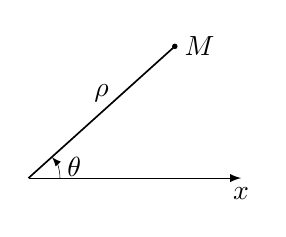
\begin{tikzpicture}[>=latex,scale=1]
  \draw[thin,->](0,0)--(2.7,0)node[below]{$x$};
  \draw[semithick](0,0)--(42:2.5)node[midway,above]{$\rho$};
  \fill(42:2.5)circle(1pt)node[right]{$M$};
  \draw[very thin,->](0:0.4)arc(0:42:0.4)node [midway,right]{$\theta$};
\end{tikzpicture}
\end{document}